\documentclass[11pt]{article}
\RequirePackage{fullpage}
%\RequirePackage[font=small,labelfont=bf]{caption}
\RequirePackage{amsmath,amssymb,amsthm}
\RequirePackage{graphicx}
\RequirePackage[hidelinks]{hyperref}
\RequirePackage{subcaption}
\RequirePackage{wasysym}
\RequirePackage{authblk}
\RequirePackage{bm}
\RequirePackage{bbm}

\RequirePackage{cleveref}
\RequirePackage{xr}
\externaldocument{supplementary}

%\RequirePackage[osf]{mathpazo}
\let\temp\rmdefault
\RequirePackage{mathpazo}
\let\rmdefault\temp

\RequirePackage[bibstyle=authoryear,citestyle=authoryear-comp,
                date=year,
                maxbibnames=9,maxnames=5,maxcitenames=2,
                backend=biber,uniquelist=false,uniquename=false,
                % style=apa,
                sorting=nyt,
                % sorting=,
                hyperref=true]{biblatex}
\RequirePackage{color}
\RequirePackage{nicefrac}

\addbibresource{biblio.bib}

% line numbers:
\RequirePackage{lineno}
%\modulolinenumbers[5]
\renewcommand\linenumberfont{\normalfont\tiny\sffamily\color{black}}

\renewcommand{\P}{\mathbb{P}}
\newcommand{\E}{\mathbb{E}}
\newcommand{\V}{\text{V}}
\DeclareMathOperator{\var}{var}
\DeclareMathOperator{\cov}{cov}


%\title{Towards a Complete Model of the Negative Selection Process in Humans}
%\title{An Evolutionary Quantitative Genetic Model of the Negative Selection Process in Humans}
\title{A Quantitative Genetic Linked Selection Model of the Negative Selection Process in Humans}

\author{Vince Buffalo and Andrew Kern}

\begin{document}
\maketitle



\begin{abstract}

    Across the human genome, there are large-scale fluctuations in genetic
    diversity caused by the indirect effects of selection. This can be thought
    of as a ``linked selection signal" that reflects selection's effects
    varying according to the placement of functional regions and recombination
    rates along the genome. Previous work has shown that negative selection
    against the steady influx of new deleterious mutations into conserved
    regions is the predominant mode of selection in humans. However, the
    theoretic model that underpins these results, classic Background Selection
    theory, is only applicable when new mutations are so deleterious that they
    cannot drift up in frequency and ultimately fix in the population. Here, we
    develop an alternate theoretic basis for genome-wide linked selection based
    on a quantitative genetics view, which considers how diversity is reduced
    according to the arrangement of additive fitness variance along the genome.
    Using a recent model that jointly predicts the equilibrium fitness variance
    and substitution rates due to deleterious mutations, we estimate the
    distribution of selection coefficients and mutation rate across three human
    populations. While our model can accommodate weaker selection, we find
    consistent evidence across all populations of very strong selection against
    deleterious mutations. We also find that our model's predicted substitution
    rates are qualitatively consistent with observed divergences in features
    under weak selective constraint like introns and UTRs, but less so in
    regions under strong selective constraint. While our model explains up to
    67\% of the out-sample variance in diversity at the megabase scale, we find
    evidence of residual strong selection against loss-of-function variants
    unfit by our model, indicating the dominant role negative selection plays
    in the human genome. Altogether, our genome-wide model of the linked
    selection is a step towards uniting population and quantitative genetic
    models of selection with the substitution processes.

\end{abstract}


\section*{Introduction}

The continual influx of new mutations into populations is the ultimate source
of all adaptations, but the vast majority of mutations either do not affect
fitness or are deleterious. Negative selection (i.e. purifying selection) works
to eliminate these deleterious mutations from the population; thus we expect
them to appear at low frequencies within populations
\parencite{Haldane1927-ga}, and be less likely to fix between lineages. The
best predictor of whether a new mutation will reduce fitness is if it occurs in
a functional region of the genome, which are often conserved over deep
phylogenetic timescales \parencite{Siepel2005-wh,Margulies2003-sn}. Since these
conserved regions reflect the product of millions of years of evolutionary
optimization, it follows that deleterious variants should be the overwhelming
majority of segregating variation in these regions. Furthermore, rare variation
in these regions is responsible for a significant portion of phenotypic
variation and disease in humans
\parencite{Zeng2018-ci,Lek2016-cb,Karczewski2020-ky,Tennessen2012-ge}.

Selection on both beneficial and deleterious variants perturbs the allele
frequencies of neighboring linked sites, a phenomenon known as linked selection
\parencite{Nordborg1996-nq,Maynard_Smith1974-zr,Barton1998-aj,Charlesworth1993-gb}.
Since deleterious variation is clustered in functional portions of the genome,
we expect linked selection to reduce levels of diversity around conserved
segments (e.g. genes, regulatory elements, etc.). The genomic arrangement of
these evolutionarily conserved regions and recombination rates create a
large-scale spatial signal of the linked selection process in genetic diversity
along the genome. Since genome-wide recombination maps and putatively conserved
segments are available for many species, there has been consistent effort to
fit models to this linked selection signal to estimate population genetic
parameters such as the strength of selection and the deleterious mutation rate
\parencite{Hudson1995-pt,McVicker2009-ax}, as well as distinguish and quantify
the roles of positive and negative selection and estimate the rate of
beneficial mutations \parencite{Elyashiv2016-vt,Murphy2022-sj}. In humans,
previous work has shown that negative selection plays the dominant role in
shaping megabase-scale patterns of diversity, with positive selection having a
nearly negligible impact \parencite{Murphy2022-sj}.

Prior work to model the reduction in linked diversity due to deleterious
mutations has largely relied on the classic Background Selection (BGS) model
\parencite{Charlesworth1993-gb,Nordborg1996-nq,Hudson1995-pt,Hudson1995-xc}.
While this model has been successful in explaining many patterns of diversity,
some its simplifying assumptions may distort inferences about the negative
selection process. First, since fixation probabilities ultimately depend on the
product of the deleterious selection coefficient ($s$) and population size
($N$), the efficacy of negative selection should depend on demography.
Unfortunately, accommodating demography into theoretic negative selection
models remains an open, difficult problem \parencite{Zeng2013-ep,Johri2020-oj}.
Second, building off classic models of mutation-selection balance
\parencite{Crow1970-wm,Kimura1966-bk}, the BGS model assumes that new mutations
are sufficiently deleterious that they are invariably driven to loss. Under
this assumption, the effect of selection is well-approximated by simply
rescaling the neutral coalescent by a reduction factor known as $B =
\nicefrac{N}{N_e}$ \parencite{Charlesworth2013-kl}. However, this simple
rescaling approach is not appropriate across parts of parameter space that are
relevant to natural populations \parencite{McVean2000-bt,Good2014-yz}. In
particular, the BGS model cannot accommodate the possibility of fixation for
mutations with $2Ns \ll 1$, leading diversity to be incorrectly predicted to
fall to zero as the strength of selection diminishes. This weak selection
problem is related to the wider problem of modeling the substitution rate of
deleterious mutation (i.e. the ``ratchet" rate) and incorporating the impact of
interference from other neighboring selected sites.

In this work, we use another class of linked selection models that derive from
quantitative genetics to address limitations of the classic BGS model. These
models express linked selection in terms of how polygenic fitness variance
creates weak genetic draft, and which increases pairwise coalescence rates.
While these models can theoretically accommodate additive fitness variance from
any source as long as its rate of change is not too rapid, we focus
specifically on a deleterious-mutations-only model of fitness variance from
\textcite{Santiago2016-mu}. This model is identical to BGS when selection
against deleterious mutations is strong, but it also correctly predicts the
reduction in diversity when selection is weak by jointly predicting the
deleterious substitution rate. We extend the Santiago and Caballero (hereafter
the SC16) model of the negative selection process so that it can be fit to
patterns of genome-wide diversity, according to the spatial distribution of
genomic features that could harbor deleterious fitness variation. Using forward
simulations, we show this model leads to more accurate estimates of the
distribution of fitness effects under weak selection. Finally, we apply our
composite-likelihood method to human population genomic data and provide new
estimates of the negative selection process in humans.

\section*{Theory}

Similar to previous work, we aim to characterize the negative selection process
through the signal left on nucleotide diversity at linked sites. Although
nucleotide diversity is a less-informative statistic than the full site
frequency spectrum, it is much easier to derive theoretic models of how linked
selection alters expected pairwise coalescence times than to describe the
entire genealogy. Still, inferences drawn from the linked selection signal
about selective processes are only as accurate as the underlying theoretic
model. Our work is motivated by a well-known limitation of classic background
selection theory: it only accurately predicts levels of linked diversity when
new mutations are strongly deleterious
\parencite{Charlesworth1993-gb,McVean2000-bt,Good2013-lp,Gordo2002-dr}.
Unfortunately, modifying background selection theory so that it accommodates
weak selection has been challenging problem
\parencite{Good2014-yz,Haigh1978-gt,Higgs1995-xc}. Here, we develop intuition
for why the classic BGS model works well for strong selection but not weak, and
how formulating the equilibrium between new deleterious mutations and negative
selection in terms of the additive fitness variance can alleviate these
problems.

Throughout, we imagine a negative selection process where a continual influx of
deleterious mutations occur at a rate of $\mu$ per basepair per generation in a
conserved region of $L$ basepairs, such that the region-wide per generation
diploid mutation rate is $U = 2 \mu L$. Each mutation imposes a selective cost
of $s$ in heterozygotes and $2s$ in homozygotes, and fitness effects are
multiplicative across sites. When selection against a new mutation is strong,
the stochastic perturbations it experiences due to random genetic drift are
weak relative to the frequency changes caused by selection. In this case, every
deleterious mutation is destined to eventual extinction, and only the fraction
of lineages without any mutations contribute to the long-run ancestry of future
populations. The classic background selection approximates this process by
rescaling the neutral coalescent with an effective population size of $N_0 = N
\exp(-\nicefrac{U}{s})$
\parencite{Charlesworth1993-gb,Nordborg1996-nq,Hudson1995-pt,Hudson1994-oh}.
This approximation works well for two reasons (though see
\cite{Cvijovic2018-vd,Walczak2012-fi,Nicolaisen2012-vs}). First, the number of
mutations per haplotype has has a stationary Poisson distribution with an
average equal to the deterministic mutation-selection equilibrium
\parencite{Haldane1927-ga}. Second, the time it takes for a present-day lineage
to trace their ancestry back to a mutation-free ancestor (the ``delay phase")
is negligible compared to the coalescence timescale of $N_0$ among
mutation-free ancestors (\cite{Durrett2008-ql}, p. 213; \cite{Good2014-yz}).

By contrast, when selection is weak, the frequency trajectories of both neutral
and selected sites are strongly impacted by stochastic perturbations from two
sources. First, genetic drift, which is due to Mendelian segregation and
non-heritable fitness differences; the magnitude of its perturbations are set
by the \emph{drift-effective} population size, $N_e$. Second, genetic draft
occurs when an allele becomes randomly associated with a fitness background
that perturbs its trajectory across generations
\parencite{Neher2013-dz,Gillespie2000-mh,Gillespie2001-mv}. Like genetic drift,
the perturbations due to draft are directionless but overall increase the
variance in allele frequency change. Unlike drift, the impact of the stochastic
perturbations due to draft are autocorrelated and build up over generations
until the fitness background recombines off
\parencite{Robertson1961-ho,Santiago1995-hx,Buffalo2019-qs}. The stochastic
perturbations due to selection also impact selected sites, and alter their
dynamics, creating Hill--Robertson interference \parencite{Hill1966-kd}. Strong
draft can generate multiple-merger coalescences that create discontinuities in
allele frequency trajectories, making diffusion approximations ill-suited
\parencite{Gillespie2000-mh,Der2011-it,Neher2013-dz}. However, when selection
is weak, draft is well-approximated as an increase in the rate of drift (or
equivalently, a reduction in effective population size).

The stochastic perturbations from genetic drift and draft impact both
genealogies and selection dynamics in complex ways, which has made finding
analytic theory predicting their joint effects difficult. When drift acts
alone, the relevant scale of perturbations is determined by the
\emph{drift-effective population size} $N_e$
\parencite{Ohta1971-gq,Ohta1992-yi}. When the random perturbations due to drift
are stronger than the changes due to selection ($2N_es \le 1$), weakly
deleterious mutations can drift up to intermediate frequencies before their
eventual loss or fixation. The assumptions of classic BGS suddenly breakdown in
two ways. First, the ``delay phase" is no longer negligible and genealogies are
no longer well-approximated by a rescaled neutral coalescence process
\parencite{Przeworski1999-mb,OFallon2010-my,Higgs1995-xc}. Second, the
distribution of the number of deleterious mutations (and its corresponding
fitness distribution) is no longer a stationary Poisson distribution, instead
becoming a traveling wave \parencite{Rouzine2008-qz,Good2013-lp,Gessler1995-hz}
towards reduced population fitness (since we ignore beneficial mutations). When
this occurs, individuals in the least-loaded class are stochastically lost,
fixing those mutations with a click of ``Muller's ratchet"
\parencite{Muller1964-ki,Charlesworth1997-qn}. Unfortunately, determining the
rate of Muller's ratchet is another difficult, open problem
\parencite{Haigh1978-gt,Gordo2002-dr,Gessler1995-hz} related to Hill--Robertson
interference \parencite{Felsenstein1974-xm}.

Our work extends theory from \textcite{Santiago2016-mu}, which suggests both
strong and weak negative selection can be be accommodated with a quantitative
genetic model of linked selection. These linked selection models stem from
\textcite{Robertson1961-ho}, which in essence describes how heritable polygenic
fitness variation generates weak genetic draft. At the individual level
Robertson considered, selection generates autocorrelation as offspring from
large families tend to beget many descendents themselves (and likewise with
small families) when fitness is heritable. This same autocorrelation occurs at
the genomic level with linkage \parencite{Santiago1998-bs,Barton2000-zg}, as
the perturbations to a neutral allele's trajectory from its particular fitness
background tend to occur in the same direction across generations until the
background recombines off. These models quantify the total impact of the
autocorrelation generated by weak draft in terms of what we think of as a
\emph{draft-effective} population size $N_d$. The key insight is that in the
long-run, steady, weak draft created by the presence of additive genetic
fitness variance $V_A > 0$ acts like an extra variance in offspring number
would under pure drift \parencite{Wright1938-tv}. However, due to
autocorrelation, the cumulative effect of this fitness variance is inflated by
a factor of $Q^2$. Intuitively, the product $V_A Q^2$ represents the expected
total variance in reproductive success a neutral mutation experiences over its
lifetime in a system with weak selection draft. 

We define the draft-effective population size $N_d$ by including the total
additional variance created by heritable fitness in Wright's
(\citeyear{Wright1938-tv}) equation for effective population size,

\begin{align}
    \label{eq:main_Ne}
    N_d = \frac{N}{Q^2 V_A + 1}
\end{align}
%
(c.f. \cite{Robertson1961-ho,Santiago1995-hx}; see Supplementary Materials Section
\ref{supp:theory} for a proof). The benefit of modeling draft with Robertson's
forward-time model is that the inflation factor is invariant with respect to
the particular fitness background the neutral allele becomes stochastically
associated with. By contrast, the difficulty with modeling draft backwards in
time is that the coalescence rates experienced by a lineage are not invariant
to which lineage was sampled due to its particular associated fitness
background.

Equation \eqref{eq:main_Ne} is general, since different modes of selection and
linkage can be accommodated by different expressions for $V_A$ and the
inflation factor $Q^2$ \parencite{Santiago1995-hx,Santiago1998-bs}. When
fitness variation has a multiplicative polygenic basis, as is often assumed for
genome-wide negative selection processes, the draft asymptotic effective
population size experienced by an arbitrary neutral site under the influence of
all linked regions is,

\begin{align}
    \label{eq:polygenic_Ne}
    N_d \approx N \exp\left(-\sum_{i=1}^S V_{A,i} \frac{Q_i^2}{2}\right)
\end{align}
%
where the factor of one-half comes from ignoring weak associations from
unlinked regions and chromosomes (see Supplementary Materials Section
\ref{supp:heritable-fitness}). In our genome-wide model, we consider the
summation in Equation \eqref{eq:polygenic_Ne} over non-overlapping segments $i
\in \{1, 2, \ldots, S\}$ each undergoing selection such that segment $i$
contributes additive fitness variance $V_{A,i}$ to the total additive genetic
fitness variance. Under equilibrium levels of fitness variation, the
autocorrelation function for a neutral allele associated with segment $i$ is
$C(t) = [(1-r_i)(1-\kappa_i)]^t$, where $r_i$ is the recombination fraction to
the segment and $\kappa_i$ is the rate that the associated fitness variance
decays due to selective dynamics. Then, the cumulative autocorrelation is,

\begin{align}
    \label{eq:Q}
    Q_i &= 1 + \sum_{j=1}^\infty \left[(1-r_i)(1-\kappa_i)\right]^j \nonumber \\
        &= \frac{1}{\kappa_i + r_i(1-\kappa_i)}.
\end{align}

(see Appendix Equation \ref{eq:Qinf}). This general equation can accommodate
models of polygenic selection as long as the equilibrium additive fitness
variation $V_{A,i}$ can be specified and the change in variance due to
selection can be approximated as a geometric decay, i.e. $\Delta V_{A,i} =
-\kappa V_{A,i}$ \parencite{Bulmer1971-ae,Keightley1988-eq,Walsh2018-bt}. This
is usually a reasonable assumption since within-generation selection removes a
fraction of phenotypic variation from the population, and some fraction of that
is additive genetic variation \parencite{Bulmer1971-ae,Keightley1988-eq}.

The remaining pieces are expressions for the equilibrium additive fitness
variance $V_A$ and the decay rate in associated fitness $1-\kappa$. At this
point, we diverge from Santiago and Caballero (\citeyear{Santiago1998-bs},
\citeyear{Santiago2016-mu}) to note that the additive fitness variation is the
sum of additive \emph{genic} fitness variance $V_a$ (i.e. due to allele
frequencies) and the fitness covariance due to linkage disequilibria between
selected sites ($\delta_{LD}$), $V_A = V_a + \delta_{LD}$. Considering only the
genic variation, at equilibrium $\Delta V_{a,i} = 0$; thus, the loss in genic
fitness each generation due to selective dynamics $-\kappa V_{A,i}$ must be
equal to the increase in fitness variation due to new mutations each generation
($V_m$) and changes in the LD term \parencite{Bulmer1971-ae}. Note that the
loss in genic fitness due to drift is not time-invariant due to the build up of
autocorrelation, and considered elsewhere in the derivation (see Supplementary
Materials Equation \ref{eq:vardecay}). Then, at equilibrium $\kappa_i =
\nicefrac{V_{m,i}}{V_{a,i}}$ (see Supplementary Materials Equation \ref{eq:Z}). 

Under any selection model, the additive genic fitness variance created by a new
mutation (at frequency $x=\nicefrac{1}{2N}$) is $2s^2 x(1-x) \approx
\nicefrac{s^2}{N}$. For the entire population of $2N$ chromosomes, the fresh
variance from mutation each generation in segment $i$ is $V_{m,i} \approx
U_is^2$ where $U_i = 2\mu L_i$ is the diploid mutation rate per generation
within the segment. Under mutation-selection balance assumed by BGS, an
$L_i$-basepair segment has genic variance $V_{a,i}^{BGS} \approx U_i s$ (see
Supplementary Materials Equation \ref{supp-eq:va_bgs}) and thus $\kappa_i^{BGS}
= s$. Substituting $V_{a,i}^{BGS}$ and $\kappa_i^{BGS}$ in Equation
\eqref{eq:polygenic_Ne} and simplifying, we have

\begin{align}
    N_d = N \exp \left( - \sum_i^S \frac{\mu L_i}{s(1 + r_i(1-s)/s)^2} \right) 
\end{align}

which is identical to the genome-wide model of background selection used in
previous studies \parencite{McVicker2009-ax,Elyashiv2016-vt,Murphy2022-sj}.
Thus, the classic background selection model is a special case of the more
general theory of Santiago and Caballero (\citeyear{Santiago2016-mu}), which
they had shown previously (\citeyear{Santiago1998-bs}).

When selection is weak, however, the additive fitness variance under the
classic BGS model is no longer accurate. \textcite{Santiago2016-mu} suggested
that this is due to the loss of fitness variation that occurs when a
segregating site fixes and its heterozygosity becomes zero. If we let $R$
represent the fixation rate (i.e. ratchet rate) in the region per generation,
each fixation removes the equivalent amount of equilibrium variation put in by
mutation. Thus, the steady-state genic variance under mutation and negative
selection is (omitting the segment index $i$ for clarity),

\begin{align}
  \label{eq:Va}
  V_{a} = (U - 2 R)s. 
\end{align}

where the condition $V_a \ge 0$ is met when the probability of fixation is less
than or equal to the neutral fixation probability of $\nicefrac{1}{2N}$, which
is held when considering deleterious mutations. This equation connects the
equilibrium additive genic fitness variance to the flux of new variation in due
to new deleterious mutations and the flux out due to their substitution and the
decline in mean population fitness. When $R=0$, selection is so strong it
cannot fix, and the equilibrium fitness variation is due entirely to young rare
mutations before their extinction $V_a = V_a^{BGS} \approx Us$. Santiago and
Caballero derive Equation \eqref{eq:Va} through Fisher's Fundamental Theorem of
Natural Selection, but we find an alternative proof (\cite{Higgs1995-xc}; see
Supplementary Materials Section \ref{supp:weak-strong}). We also find that the
steady-state additive genic variance in Equation \eqref{eq:Va} results from
diffusion models with a flux of mutations into discrete sites
(\cite{Kimura1969-jw}). 

%Our results differ from \parencite{Santiago2016-mu}, since we find from
%simulations their expression models the additive \emph{genic} fitness
%variation, not additive genetic fitness variation (see Section XXX). This is
%because Equation \eqref{eq:Va} does not capture the expected build-up of
%negative linkage disequilibria when selection is mildly deleterious.

While using Equation \eqref{eq:Va} in Equation \eqref{eq:main_Ne} leads to a
prediction for the draft-effective population size $N_d$, closed-form
expressions for the rate of the ratchet $R$ have generally been hard to find
\parencite{Haigh1978-gt,Higgs1995-xc,Gessler1995-hz}. The key insight of
\textcite{Santiago2016-mu} is that the ratchet rate under draft is determined
by the probability of fixation $p_F(N_d, s)$
\parencite{Kimura1962-su,Malecot1952-qh} using the draft-rescaled effective
population size, i.e. $R = N U p_F(N_d, s)$. Given this equation for the
ratchet and Equation \eqref{eq:polygenic_Ne} for $N_d$ under draft, we have a
system of two non-linear equations that can be solved numerically for $N_d$ and
$R$ for each segment,

\begin{align}
  \label{eq:main_eqns}
  N_d &= N \exp \left( -(U-R)s \frac{Q^2}{2} \right) & \text{\emph{draft-effective population equation}} \\
  R &= \frac{4N_d U s}{\exp(4 N_d s)-1}  & \text{\emph{ratchet equation}}
\end{align}
%

We denote the solutions to these equation, which represent equilibria under
mutation-selection-drift-draft process, as $\widetilde{N}_d$ and
$\widetilde{R}$. These equilibria also imply an equilibrium level of additive
fitness variation $\widetilde{V}_a$ in the segment, which are used to calculate
the reduction factor $B(x) = \nicefrac{N_d}{N}$ at any genomic position $x$
(see Methods \ref{sec:methods-maps}).

\section*{Results: Simulation Validation of Theory and Methods}

Given that modeling the interplay of mutation, drift, and draft under both weak
and strong selection has proven to be difficult problem, we first sought to
verify the SC16 theory and our genome-wide extension of this theory with three
levels of simulations: forward simulations of negative selection in a region,
chromosome-scale forward simulations of negative selection, and simulations of
a ``synthetic genome" to test our composite-likelihood method based on this
theory.

\subsection*{Simulations of a Segment under Negative Selection}
\label{sec:segment-sims}

\begin{figure}[htbp] \centering
    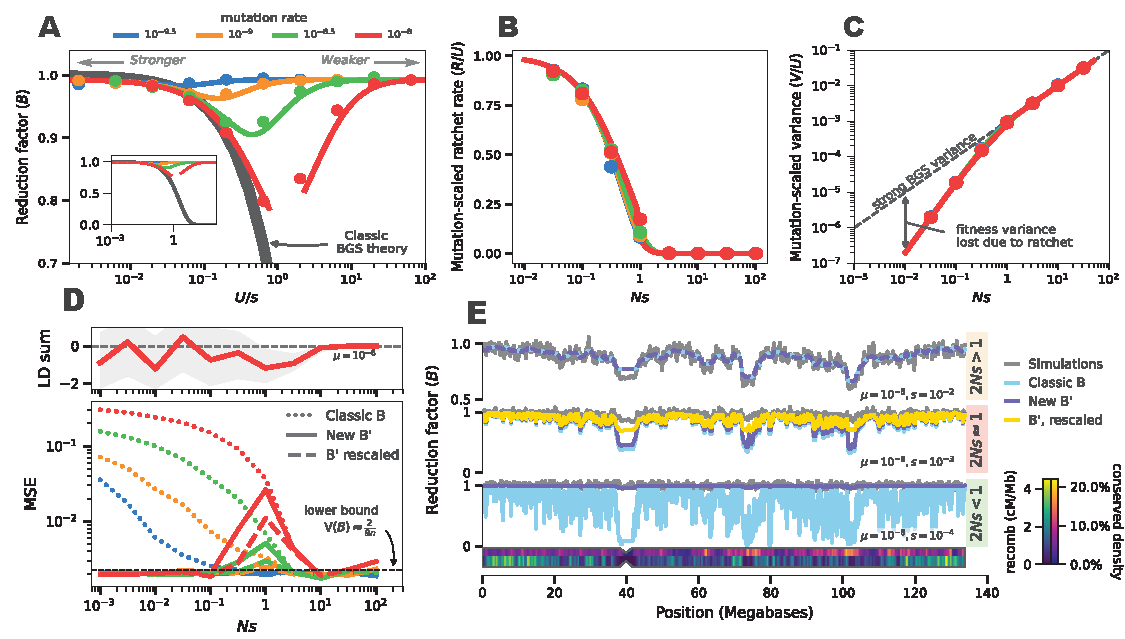
\includegraphics[width=\textwidth]{figures/figure_1.pdf} \caption{Theory
        compared to simulation results. (A) The predicted reduction factor
        under classic B theory (dark gray line) and the diploid SC16 model
        (colored lines corresponding to mutation rate) compared to average
        reduction across 10,000 simulation replicates (points). (B) The predicted
        ratchet rate under the SC16 model scaled by mutation rate (colored
        lines) compared to the ratchet estimated from simulation (points). When
        $2Ns>1$, the ratchet rate is near zero. (C) The genic variance from
        simulations (points) against the predicted variance under the SC16
        model (colored lines). As the ratchet begins to click, the genic
        variance is decreased from the level expected under strong BGS (dashed
        line). (D, bottom) The mean squared error (MSE) between
        whole-chromosome simulations and predicted classic B (dots), new B'
        (solid), and locally-rescaled B' (dashed) for different mutation rates
        (colors). The dashed horizontal line is the approximate theoretic
        minimum MSE. (D, top) The build up of negative linkage disequilibria
        around $2Ns=1$ in whole-chromosome simulations in bottom panel. (E) The
        average B map from 100 chromosome 10 simulation replicates (gray)
    against different predictions, for parameters that correspond to $2Ns < 1$,
$2Ns = 1$, and $2Ns > 1$. The chromosome shows the density of conserved sites
and recombination map used in simulations. }
  \label{fig:figure-1}
\end{figure}

Our first set of forward simulations were to ensure that the SC16 model
adequately captures selective dynamics in a single $10^5$ basepair region
undergoing negative selection, across a variety of mutation rates and selection
coefficients (see Methods \ref{sec:methods-sim}). We find a close
correspondence between the observed and predicted reductions in effective
population size $B=\nicefrac{N_d}{N}$ over all selection and mutation
parameters including weak selection (Figure \ref{fig:figure-1}A), in contrast
to classic BGS theory. Furthermore, to investigate whether this accuracy was
caused by the model correctly predicting the equilibrium fitness variance and
ratchet rate, we also measured these throughout the simulation. Again, we find
the diploid SC16 theory accurately predicts both the ratchet rate (Figure
1\ref{fig:figure-1}B) and the genic fitness variance (Figure
1\ref{fig:figure-1}C).

Moreover, these simulations provide intuition about the underlying negative
selection process. When mutations are strongly deleterious, there is no chance
they can fix, and the ratchet rate is zero (Figure \ref{fig:figure-1}B for $2Ns
> 1$). In this strong selection regime, the additive genic fitness variation
closely matches the theoretic deterministic equilibrium of $V_a = Us$ (dashed
gray line, Figure \ref{fig:figure-1}C) However, around $2N_e s \approx 1$, the
ratchet begins clicking as $p_F > 0$. When this occurs, each click of the
ratchet eliminates variation, and the equilibrium variation diverges from the
deterministic mutation-selection equilibrium (Figure \ref{fig:figure-1}C).

\subsection*{Chromosome-wide Simulations and Models of Negative Selection}
\label{sec:chrom-sims}

Given the accuracy of the SC16 model in predicting the reduction factor $B$ and
ratchet rate for a single segment under general mutation-selection processes,
we next extended their model so that it could be applied to whole-genome data.
Our software method \texttt{bgspy} numerically solves Equations
\eqref{eq:main_eqns} to compute the equilibrium additive genic fitness variance
($V_a$) and ratchet rate ($R$) across grids of mutation rates and selection
coefficients. This is done for each pre-specified segment in the genome that
may be under negative selection (e.g. coding sequences or UTRs). Then, these
equilibrium can be used to calculate a reduction map $B(x)$ across genomic
positions $x$. To distinguish between McVicker's B maps based on classic BGS
theory, we call our reduction map $B(x)$ a B' map.

We validated our predicted B' reduction maps with realistic chromosome-scale
forward simulations of negative selection in conserved regions. Averaging over
$100$ replicates, we estimated the simulation empirical reduction map and
compared this to the predicted B and B' maps for the same parameters. We find
that our B' maps and the classic BGS theory B maps closely match simulations
when selection is strong (top row of Figure \ref{fig:figure-1}E). This provides
the first realistic forward-time chromosome-scale simulation confirmation of
classic BGS theory. However, we find slight discrepancies in regions with low
recombination (Figure \ref{fig:figure-1}E). Second, we find our theory is
vastly more accurate than the classic B maps when selection is very weak ($2N_e
s \ll 1$; bottom row of Figure \ref{fig:figure-1}E), which is expected since
BGS theory does not work in this domain. Across all mutation and selection
parameters simulated, the relative error of the classic B maps is 14.6\%
whereas the relative error in the new B' maps is 5\%. Additionally, we find
that the mean squared error between simulations and B' maps is close to the
theoretic lower bound set by the coalescence variance
\parencite{Tajima1983-gu}.

The discrepancy between our theoretic B' maps and chromosome-wide simulations
that leads to the 5\% error occurs entirely around the drift-barrier domain of
$2Ns \approx 1$ (Figure \ref{fig:figure-1}D). The higher error in this domain
occurs across all mutation rates. We hypothesized this error may be due to
selective interference between segments that is not taken into account when we
numerically solve Equations \eqref{eq:main_eqns} for each segment
independently. In particular, we use a fixed drift-effective $N=1000$
corresponding to the number of diploids in the simulations rather than $B(x) N$
at position $x$. To test this, we implemented a ``locally-rescaled" version of
the B' maps, which numerically solves Equations \eqref{eq:main_eqns} for each
segment at position $x$ taking into account the reduction experienced due to
selection at other segments by setting $B'(x)N$ as the population size. We find
the locally-rescaled B' maps reduce the relative error from 5\% to 0.4\% and
mean squared error (Figure \ref{fig:figure-1}D, dashed colored lines), but does
not entirely eliminate the error in the $2Ns \approx 1$ domain. Overall, while
we find evidence that local-rescaling slightly reduces error in the $2Ns
\approx 1$ domain, we do not use it during in our genome-wide inference method.
This is because to avoid circularity and possible overfitting, our method would
need to solve the equilibria equations for all segments simultaneously;
unfortunately, this is currently computational unfeasible.

Finally, we hypothesized that the remaining error is because of the build up of
negative linkage disequilibria between selected sites due to Hill--Robertson
interference \parencite{Hill1966-kd,McVean2000-bt,Comeron2007-wq}. To assess
this possibility, we calculated the sum of all linkage disequilibria in our
chromosome-wide simulations. We find negative linkage disequilibria build ups
around $2Ns \approx 1$ (Figure \ref{fig:figure-1}D, top row) and is stronger
when mutation rates are higher. As $Ns \to 0$, the variance in LD inflates as
expected \parencite{Ohta1969-ae,Hill1968-ue}. Overall, the build up of negative
LD is consistent our view that the equilibrium fitness variance modeled by the
SC16 theory is the additive \emph{genic} fitness variance, which differs from
the additive genetic variance by the sum of linkage disequilibria between
selected sites (i.e. $\delta_{LD} = s^2 \sum_{i\ne j} D_{i,j}$ where $D_{i,j}$
is the LD between sites $i$ and $j$). However, according to theory, the
reductions in diversity should be determined by levels of additive genetic
fitness variance that include the contribution of LD (Supplementary Materials
Section \ref{supp:theory}).

\subsection*{Validation of Composite-likelihood Method using Forward
Simulations}

\begin{figure}[htbp] \centering
    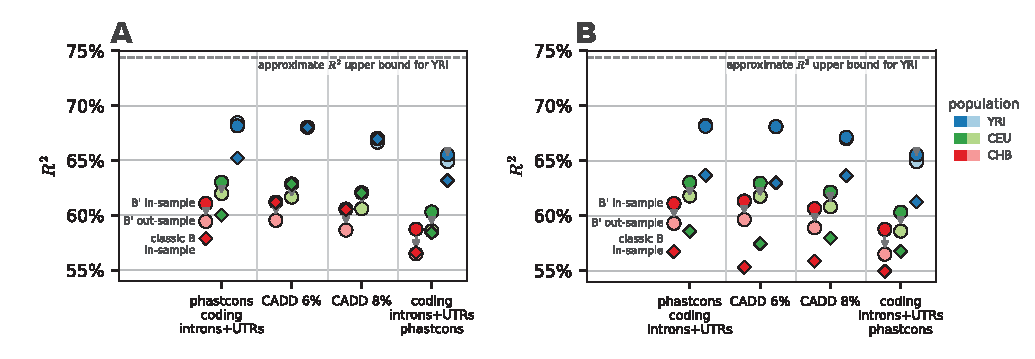
\includegraphics[width=0.8\textwidth]{figures/figure_2.pdf} 
    \caption{Comparison of parameter estimates using classic BGS theory (green
        lines) with our new B' method (blue lines) across both full and sparse
        track types (dark versus light hue), and different mutation rates
        (columns). In the first row, $R^2$ between predictions and observations
        increases with selection intensity. Both classic BGS and B' methods fit
        the data equally well with sparse tracks, though the estimated
        selection coefficients are inaccurate when selection is weak (second
        row). Mutation rate estimates (third row) are more accurately estimated
        by the B' method than classic BGS, but overall show slight biases.
        Overall, classic BGS methods fail as expected when full-coverage tracks
    are used, since it cannot accommodate weak selection and neutrality. }
  \label{fig:figure-2}
\end{figure}

We next developed a composite-likelihood method that estimates the distribution
of selection coefficients for each feature type, the mutation rate, and the
diversity in the absence of linked selection ($\pi_0$) by fitting the theoretic
reduction map to genome-wide diversity (see Methods
\ref{sec:methods-likelihood}). We validated that our method can accurately
estimate the parameters of negative selection by simulation a ``synthetic
genome" of the first five human chromosomes (see Methods
\ref{sec:methods-sim}). We note three findings from these simulations.

First, we find the $R^2$ between predicted and simulated megabase-scale
diversity serves as a measure of the strength of the linked selection signal in
genome-wide data. The $R^2$ increases with the intensity of selection against
new deleterious mutations and mutation rate (Figure \ref{fig:figure-2}, top
row). Under just drift or weak negative selection, the variance in diversity is
driven by unstructured coalescence noise along the genome and the predicted
reduction map $B(x)$ does not fit the data well. However, we note that under
very strong selection ($s=0.05$), $R^2$ is reduced. This is like due to very
strong selection having less localized effects and impacting overall
genome-wide diversity \parencite{Santiago1995-hx,Robertson1961-ho}.

Second, both our implementation of classic BGS theory and our B' method
accurately infer the average selection coefficient under strong selection
(Figure \ref{fig:figure-2}, middle row). However, when selection was weak, the
classic BGS model erroneously estimates strong selection and a very low
mutation rate. By contrast, our B' method estimated selection coefficients much
closer to their true value. A minor discrepancy occurs around $2Ns = 1$, likely
due to the sensitivity of mutations in this region to selective interference
(discussed in Section \ref{sec:chrom-sims}). Because we only simulated fixed
selection coefficients and five chromosomes, we only assessed the accuracy of
average selection coefficients and not the DFE probabilities.

Third, we find slight biases in mutation rated estimated by both our B' and the
classic BGS methods (Figure \ref{fig:figure-2}, bottom row). However, mutation
rate estimates based on our B' method are more accurate than classic BGS theory
across a range of selection coefficients. Overall, the bias in estimated
mutation rates suggests that benchmarking genome-wide negative selection models
based on their agreement with pedigree-based rate estimates may not be
appropriate. When BGS is not functioning, either due to weak selection or a low
rate of deleterious mutations (Figure \ref{fig:figure-2}, right column), all
estimates deteriorate. This is understandable, as the overall signal from
linked selection weakens relative to drift-based noise. We should note, though,
that this is an unlikely region of parameter space and this issue can be
readily diagnosed from the low $R^2$ values.

Finally, we tested the sensitivity of our method to violations of two
assumptions---constant population size and recessivity of selective
effects---through simulations. Using an expansion rate and timing as estimated
for Europeans by \textcite{Gutenkunst2009-pg}, we found that a population
expansion had minimal impact on parameter estimates (Supplementary Materials
Section \ref{supp:sim-assum}). We did not test the influence of population
bottlenecks, since parameter estimates of out-of-Africa bottlenecked
populations (CHB and CEU) did not differ much from YRI estimates (see below).
However, these simulations did find that selection coefficient estimates were
downwardly biased when deleterious mutations were recessive and weak.
Recessivity did not bias selection coefficient estimates when selection was
strong; this is expected since strongly deleterious mutations are predominantly
are sufficiently rare that they are not often found in a homozygote. Overall,
the sensitivity to recessivity is likely due to the ratchet rate being
overestimated when selection is weak and recessive mutations drift up to higher
frequency and experience stronger than expected selection in homozygotes.

\section*{Results: Application to Human Genomic Data}

\subsection*{Annotation Model Comparison}
\label{sec:annotation}

Our composite likelihood method takes tracks of annotated features (an
``annotation model") that are \emph{a priori} expected to have similar fitness
effects, and estimates the overall mutation rate and distribution of fitness
effects for each feature type. We consider two classes of annotation models:
(1) CADD-based models, which consider the top $x\%$ most pathogenic basepairs
according to the CADD score, and (2) and more interpretable gene feature-based
models that includes protein coding regions, intron and UTRs, and PhastCons
regions. We include PhastCons regions because there is strong evidence of
highly-conserved non-coding regions
\parencite{Meader2010-hm,Harmston2013-tt,Katzman2007-gq,Siepel2005-wh}, that
would be missed by gene feature only annotation. These two classes of
annotation models have a trade-off between fine-scaled specificity to which
basepairs are likely to be under negative selection, and interpretability of
the DFE estimates for each feature.

Our method estimates the distribution of fitness effects (DFE) for each feature
class. While CADD-based models only have a single conserved feature class (e.g.
CADD 6\%), feature-based models can have multiple feature classes under varying
levels of selective constrain. However, overlapping features (e.g. a basepair
that is annotated as both PhastCons and coding sequence) must be assigned to
one category or the other. Since this assignment impacts DFE estimates, we fit
both of the two alternative models. First, a \emph{PhastCons Priority} model,
where genic features that overlap PhastCons regions are classified as
PhastCons, and all remaining coding basepairs are labeled as CDS. Second, a
\emph{Feature Priority} model, where all coding basepairs are assigned to CDS,
and the PhastCons class catches the remaining highly-conserved non-genic
regions. 

In total, we fit four annotation models (CADD 6\%, CADD 8\%, PhastCons
Priority, and Feature Priority) to high-coverage 1000 Genome data for three
populations: Yoruba (YRI), Han Chinese (CHB), and European (CEU) reference
samples. We assess and compare our models according to how well they predict
patterns of diversity on whole chromosomes left-out during the model fitting
process (e.g. leave-one-chromosome-out, LOCO). We use the metric
$R_\text{LOCO}^2$, which is the proportion of the observed variance in genomic
diversity at the megabase scale predicted by our model. We experimented with a
few smaller spatial scales (e.g. 100 kbp), but our results were consistent with
previous results suggesting the human linked selection signal fits best at the
megabase scale \parencite{Murphy2022-sj}.

\begin{figure}[htbp] \centering
    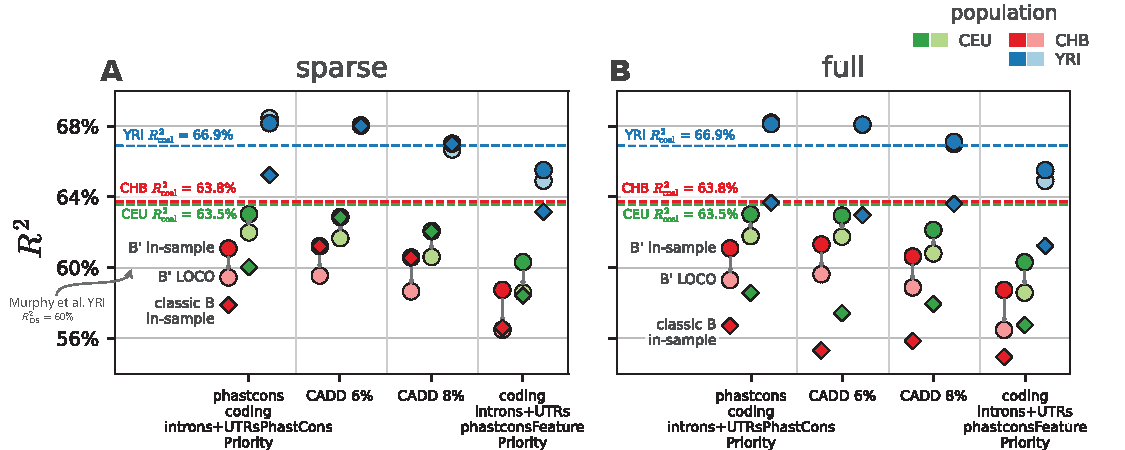
\includegraphics[width=\textwidth]{figures/figure_3.pdf} 

    \caption{The $R^2$ estimates for a sparse (A) and full (B) models, for all
        populations (colors) fit at the megabase-scale. Round points are our B'
        method and diamonds are the classic BGS (we exclude classic BGS in the
        full track subfigure, since these all fit very poorly). Lighter color
        round points are the out-sample $R_\text{LOCO}^2$ estimates for our B'
        method, and arrows show the decline in goodness-of-fit due to in-sample
        overfitting (out-sample $R_\text{LOCO}^2$ were not calculated for
        classic B values due to computational costs). The horizontal dashed
        lines are the $R_\text{drift}^2$ expected when the residual variance is
    given by the theoretic variance in coalescence times due to drift alone.}

  \label{fig:figure-2}
\end{figure}

Overall, we find the PhastCons Priority and CADD 6\% models fit about equally
as well (Figure \ref{fig:figure-2}A), consistent with recent work using classic
BGS theory \parencite{Murphy2022-sj}. However, we find that our models predict
out-sample diversity levels slightly better than previous methods. For these
two models, we find that our B' method predicts $R_\text{LOCO}^2=67.3$\% and
$R_\text{LOCO}^2=66.7$\% of the out-sample variance in Yoruba pairwise
diversity at the megabase-scale, respectively. By contrast, the best-fitting
CADD 6\% model from \textcite{Murphy2022-sj} explained 60\% of diversity in
left-out 2 Mbp windows across YRI samples. We note that this difference could
be explained by other differences in data processing, optimization, etc. For
populations impacted by the out-of-Africa bottleneck, the goodness-of-fit was
lower across all models (e.g. 61.0\% and 58.8\% for CEU and CHB respectively in
the PhastCons Priority model).

Our PhastCons Priority model fits marginally better than the CADD 6\% model
consistently across all three populations (Supplementary Table
\ref{supp:tbl-r2}). This is likely because the PhastCons Priority model has
more DFE parameters, and thus can fit finer-scale differences among the four
feature types. By contrast, the CADD 6\% track must fit patterns of diversity
to conserved sites under a single DFE. The CADD 8\% model fit slightly worse
than the CADD 6\% across all populations, and the Feature Priority model had
the poorest-fit.

Since our method is built upon theory that fixes the weak selection problem of
classic BGS theory, it should in principle fit equally well when an annotation
model includes regions that are under no selective constraint and thus
neutrally evolving. To test this, for each of our annotation models (which are
``sparse") we fit a corresponding ``full" model that assigns the remaining
portion of the genome to a feature called ``other". Ideally, how a model fits
using our B' method should be invariant to whether an annotation model is
sparse or full, since our method in principle can accommodate weak selection
and neutrality. Indeed, we find this to be the case: both in-sample $R^2$ and
out-sample $R_\text{LOCO}^2$ values are nearly identical across full and
sparse-track models (Figures \ref{fig:figure-2}A and \ref{fig:figure-2}B, round
points). 

By contrast, full annotation models fit poorly under classic BGS theory, and
lead to unreasonable parameter estimates (discussed in Section XXX).
Additionally, when sparse annotation models contain genomic features that are
likely under weak constraint (such as introns and UTRs), models fit worse under
classic BGS theory than our B' method (Figure \ref{fig:figure-2}A). However,
among the CADD annotation models, the goodness-of-fit is nearly identical
between B' and classic BGS methods. This behavior is what we would expect given
that the CADD models contain only the most pathogenic sites, which are \emph{a
priori} very likely under the strong selection domain under which B' and
classic BGS theory agree.

Overall, our $R_\text{LOCO}^2$ estimates suggest our negative selection model
explains up to 67\% of out-sample variance in diversity of the megabase scale,
even though our method assumes constant demography and homogeneous mutation
rates along the genome. A worthwhile question is: how much variation
\emph{could} we expect to fit at this scale? Given that selection alters
genealogies in ways beyond just decreasing mean pairwise coalescence time and
populations have non-constant demography, an exact analytic answer is
intractable. However, we can get an approximate idea if we assume that the
residual variance $\sum_b (\pi_b - \widehat{\pi}_b)^2$ is determined entirely
by the expected neutral coalescence noise around the expected coalescence time
$2B(b)N$. This can be be found analytically, plugging-in our predictions for
$B(b)$. This allows us to calculate $R_\text{coal}^2$ to ballpark the theoretic
variance that is capable of being explained, assuming this coalescence-only
noise process (see Supplementary Materials \ref{supp:r2-coal}). We note that
selection is expected to \emph{decrease} the variance in coalescence times
beyond a rescaled effective population size implies; our $R_\text{coal}^2$
would be an underestimate under selection.

We find that our out-sample $R_\text{LOCO}^2$ for the Yoruba samples
($R_\text{LOCO}^2 \approx 67$\%) is slightly above the theoretic
$R_\text{coal}^2 \approx 66.6$\%. This suggests our model is in the vicinity of
fitting all the signal possible, under the coalescence-only noise assumption.
By contrast, for bottlenecked out-of-Africa populations, we find a larger
discrepancy between $R_\text{coal}^2$ and observed out-sample
$R_\text{LOCO}^2$. The theoretic $R_\text{coal}^2 \approx 63\%-64$\% for both
populations, compared to the observed $R_\text{LOCO}^2 \approx 61$\% for CEU
and $R_\text{LOCO}^2 \approx 59$\% for CHB under the PhastCons Priority model.
Given that bottlenecks would act to increase the residual variance in
coalescence times beyond the level implied by the effective population size,
this gap would likely shrink under more realistic models or simulation-based
approximations for $R_\text{coal}^2$. Overall, this suggests that negative
selection models explain the vast majority coalescence time variation at the
megabase-scale that is capable of being explained (i.e. that is not coalescence
noise).

\subsection*{Estimated Distribution of Fitness Effects}

\begin{figure}[htbp] \centering
    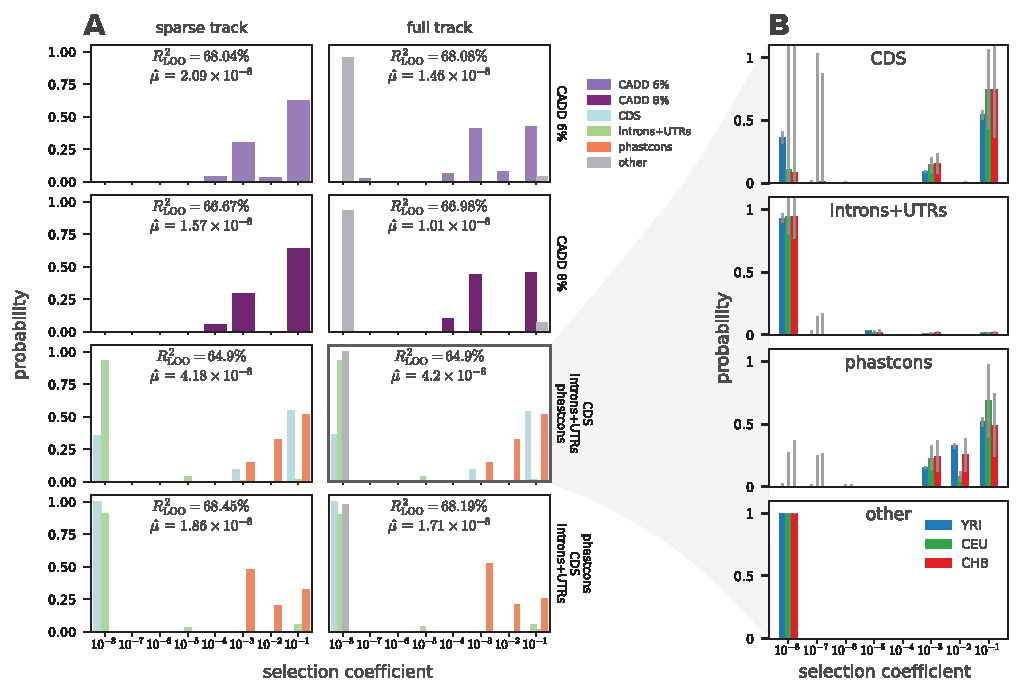
\includegraphics[width=\textwidth]{figures/figure_4.pdf} 

    \caption{The distribution of fitness effects of new mutations estimates for
        YRI reference samples. (A) The DFEs using sparse (left column) and
        full-coverage (right column) tracks, across different annotation models
        (row). Color indicates the feature type. (B) The DFE of the
    full-coverage Feature Priority model comparing the estimates across
populations. Although this model fit the data less well than alternatives, its
results are more interpretable.}

  \label{fig:figure-3}
\end{figure}

Our composite likelihood method has three sets of parameters: the expected
diversity in the absence of linked selection diversity $\pi_0$, the mutation
rate $\mu$, and the matrix of distribution of fitness effects $\mathbf{W}$
across the selection grid for each of the $K$ feature types. Given that the
relationship between $\pi$ and the strength selection is U-shaped, we wondered
whether our new B' model accommodating weak selection could fit the linked
selection signal under a different combination of weak and strong selection
parameters than found by previous work.

However, across all of our annotation models, new deleterious mutations in
conserved feature classes (CADD tracks, CDS, and PhastCons regions) were
consistently estimated to have strongly deleterious effects (Figure
\ref{fig:figure-4}A), consistent with previous work
\parencite{McVicker2009-ax,Murphy2022-sj}. The DFE estimates for CADD and
PhastCons regions consistently places $\ge 75\%$ of mass on the largest
selection coefficient, $s=10^{-2}$. The CADD 6\% DFE estimates imply an average
selection coefficient of $\bar{s} = 0.65\%$ for CEU, $\bar{s} = 0.57\%$ for
CHB, and $\bar{s} = 0.79\%$ for YRI. Similarly, the PhastCons Priority model
implies average selection coefficient estimates of $\bar{s} = 0.63\%$, $\bar{s}
= 0.59\%$, and $\bar{s}= 0.77\%$ for CEU, CHB, and YRI respectively for
PhastCons regions. Our DFE estimates for the Feature Priority model are
qualitatively consistent with the U-shaped DFEs found for amino acids through
Poisson Random Field method \parencite{Boyko2008-tj}.

Following previous work, our method used a grid of selection coefficients up to
$s=10^{-2}$. However, we also experimented with a strong selection grid that
includes $s=10^{-1}$. We find that models fit with the strong selection grid
had $R_\text{LOCO}^2$ that were about one percentage point higher, which is
suggestive of stronger selection than has previously been estimated using
constrained grids (see Supplementary Materials Table
\ref{supp:tbl-r2-strongsel}). For this strong selection grid, we estimate
average selection coefficients for the CADD 6\% model of $\bar{s} = 4.2\%$ for
CEU, $3.2\%$ for CHB, and $4.4\%$ for YRI. Thus, there is quite a degree of
sensitivity to DFEs and average selection estimates based on the selection
coefficient grid.

However, across the strong selection grid runs, we find indications of model
non-identifiability. First, estimates of the DFE with the strong grid are
strangely bimodal (Supplementary Figure \ref{suppfig:strong-sel-dfe}). For
example, under the CADD 6\% strong selection grid model, new mutations are
estimated to have a selection coefficients of $s = 10^{-1}$ with 43\% chance,
$s=10^{-2}$ with 7.8\% chance, and $s=10^{-3}$ with 41\% chance in the YRI
samples. We propose that one mechanism for this non-identifiability is that
very deleterious mutations lead to larger whole-genome reductions, which are
difficult to distinguish from a smaller drift effective population size (i.e.
the $\pi_0$ parameter). One way to test this hypothesis is to look to see if
there is a systematic positive relationship across models between average
selection coefficient and $\pi_0$, which is includes the drift-effective
population size $N_e$.

We find this is the case for all of our CADD 6\% models. Across all
populations, average selection was about $7.1$ times larger using the strong
selection grid, and $\pi_0$ was $5.6\%$ higher (see Supplementary Materials
Figure \ref{suppfig:sel-ident}). There was no similar consistent change in
mutation rate estimates among populations. In the CADD 6\% model, genome-wide
average reduction factor $\bar{B}$ was $\approx 6.1\%$ lower in the default
versus constrained grid. Overall, this suggests that the linked selection
signal alone cannot differentiate very strong selection from a slightly smaller
drift-effective population size. 

Given that it is debated how strongly demography impacts the deleterious
mutation load
\parencite{Torres2018-ni,Torres2020-hc,Lohmueller2008-qi,Simons2014-sv,Simons2016-cs},
we were curious how consistent our DFE estimates are across populations.
Overall, we find DFE estimates are relatively stable across populations and
models (Supplementary Materials Section \ref{supp:fits}). Only in our Feature
Priority model (Figure \ref{fig:figure-4}B, top row) do we see a slightly
different DFE estimate for coding sequences between YRI and CEU/CHB
populations, but this could be due to the poorer fit this model has to data.

Although the Feature Priority model fits the data less well than alternative
models, its DFE estimates are are more interpretable. We find that our B'
method estimates a bimodal DFE for coding sequences for the Feature Priority
model, with a large mass placed on $10^{-3} \le s \le 10^{-2}$ and another on
the neutral class $s=10^{-8}$. This is expected, given that the synonymous and
non-synonymous sites that constitute coding sequences are under vastly
different levels of constraint. Moreover, features expected to be only weakly
constrained such as introns and UTRs have the bulk of DFE mass on the neutral
class, with a small but significant amount of mass ($\approx 3\%$) placed on
$s=10^{-2}$. As expected, the DFE for PhastCons regions (which in this model
correspond to highly-conserved non-coding elements) suggests it is under strong
selective constraint; however we note that block jackknife based uncertainty
estimates suggest the model is uncertain whether there is some mass on the
neutral class. Finally, we highlight one result from our PhastCons Priority
annotation model (Figure \ref{fig:figure-3}A bottom row): the DFE estimate for
coding sequences excluding PhastCons regions is estimated as neutral. This too
is expected; the selection signal in coding regions is absorbed by the
PhastCons feature, leaving only conditionally neutral sites.

\subsection*{Estimates of the Deleterious Mutation Rate in Humans}

\begin{figure}[htbp] 
    \centering
    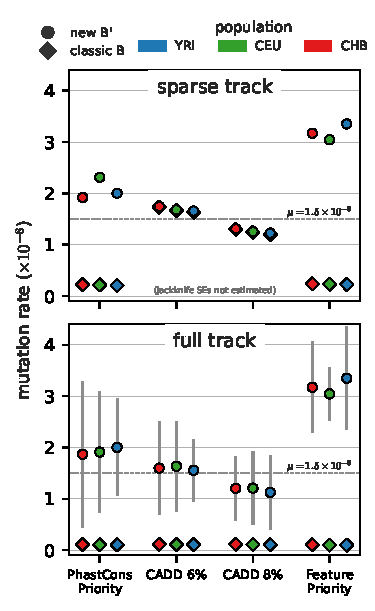
\includegraphics[width=0.5\textwidth]{figures/figure_5.pdf} 
    
    \caption{Mutation rate estimates across sparse track (top row) and
        full-coverage track (bottom row) models, for the new B' (circles) and
        classic BGS (diamonds) methods. Estimates of the mutation rate are
        consistent between classic BGS and B' methods for sparse tracks CADD
        models (overlapping diamonds and circles, top row). Overall, mutation
        rate estimates are sensitive to the underlying annotation model.}
  \label{fig:figure-4}
\end{figure}

Prior work on genome-wide inference using the classic BGS model fit the linked
selection signal well, but led to unusually high estimates of the mutation rate
\parencite{McVicker2009-ax}. This lead to the hypothesis that these models
could be absorbing the signal of positive selection \parencite{Enard2014-kz},
though other work has found a limited role for hitchhiking
\parencite{Pickrell2009-tt,Hernandez2011-gs,Murphy2022}. While our simulation
results suggest estimates of the mutation rate from linked selection models are
biased, we still check for rough agreement with pedigree-based estimates
\parencite{Kong2013-fc,Tian2019-so}. 

We find across all populations, our mutation rate estimates from CADD-based
models are roughly consistent with pedigree-based estimates (Figure
\ref{fig:figure-4}A), consistent with recent work \parencite{Murphy2022-sj}.
Our full-track CADD 6\% model estimates the mutation rate as $\widehat{\mu} =
1.56 \times 10^{-8}$ for YRI, $1.64 \times 10^{-8}$ for CEU, and $1.60 \times
10^{-8}$ for CHB reference samples (Supplementary Table \ref{supp:tbl-r2}). As
expected, the sparse-track CADD model mutation rate estimates are nearly
identical between the B' and classic BGS methods (Figure \ref{fig:figure-4}A
top row).

However, mutation rate estimates for feature-based annotation models are
implausibly higher than pedigree-based estimates. First, mutation rate
estimates under our implementation of classic BGS theory are an order of
magnitude below the expected range (Figure \ref{fig:figure-4}A top row). We
observe similar behavior when we use the classic BGS model to fit full-coverage
annotation models (Figure \ref{fig:figure-4}A bottom row). This behavior is
consistent with classic BGS theory being unable to fit the DFE to features
under weak constraint (e.g. introns, UTRs, and the ``other" feature), and most
compensate by estimating an unusually low mutation rate.

Second, we noticed that across all populations and sparse/full tracks, the CADD
6\% model consistently led to slightly higher mutation rates than the CADD 8\%
model (Figure \ref{fig:figure-4}A bottom row; Supplementary Table
\ref{supp:tbl-r2}). This same pattern was observed in Murphy et al. too (2023;
Appendix 1, Figure 16). This behavior suggests a non-identifiability issue
between a slightly higher per-basepair mutation rate and annotation tracks that
contain more conserved sequence. This is expected from theory, since both
classic BGS and SC16 models only depend on mutation rate through the compound
parameter $\mu L$, where $L$ is the length of the conserved segment. Even
though our method is much more robust to inclusion of non-conserved regions
like introns, we still observe this non-identifiability issue.

Finally, we note that mutation rate estimates in the Feature Priority model are
unreasonably high ($\widehat{\mu} \approx 3 \times 10^{-8}$), reminiscent of
the high mutation rate estimates found under McVicker et al.'s
(\citeyear{McVicker2009-ax}) model. While both our and Murphy et al.'s CADD and
PhastCons-based models alleviate this issue, it is worth discussing why this
could occur. We gain some insight from comparing the estimated mutation rates
between our Feature and PhastCons Priority annotation models, which both
contain the exact same number of feature basepairs, but these are assigned to
different feature classes based on the priority of overlapping features. That
one of these models is our best-fitting model, and the other our worst
indicates the sensitivity these models have when features classes have
heterogeneous DFEs. CADD-based models fit better in part due to their
fine-scale resolution of selective effects across the genome. While ideally we
would fit a CADD model with different features corresponding to the different
percentiles of pathogenicity, these features are on the basepair scale and thus
too memory-intensive for our method to currently accommodate.

\subsection*{Predicted Diversity and Residual Signal}

\begin{figure}[htbp] \centering
    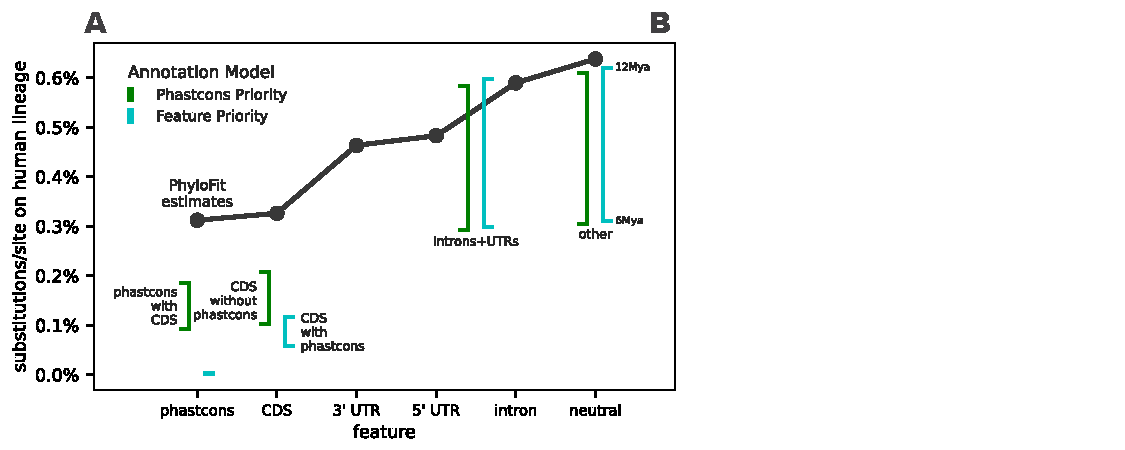
\includegraphics[width=\textwidth]{figures/figure_6.pdf} 

    \caption{(A) Observed and predicted diversity under the CADD 6\% full-track
        model. Once scaled by average diversity, populations differ little in
        their predicted diversity levels (colors). Additionally, we show
        summaries of CADD density and recombination rate along the chromosome
        below. (B) Predicted $B$ and observed $\pi$ for each window. The
        residual variance is in the vicinity of the levels expected from the
        $R_\text{LOCO}^2$ calculation. (C) Evidence that negative selection
    signal remains in CADD 6\% residuals (YRI shown). Residuals are plotted
against the average LoF selection coefficient across genes in a megabase window
(estimated by \cite{Agarwal2023-un}).}

  \label{fig:figure-5}
\end{figure}

While we have previously shown that out-sample predicted diversity matches
observed diversity (Section \ref{sec:annotation}), we also investigated whether
there were regions of the genome that were particularly poor-fitting. Comparing
predicted against observed diversity along chromosomes (see Supplementary
Materials Section \ref{supp:chrom-fit}) we find a close correspondence
consistent with the high $R_\text{LOCO}^2$. However, we find a few large (tens
of megabases) regions with systematically poorer fit (Supplementary Materials
Figure \ref{supp:spatial-residuals}). In Figure \ref{fig:figure-5}A we see one
such region on the short arm of chromosome 2, from 30 Mbp to 60Mbp.
Interestingly, predicted diversity closely follows the peaks and troughs of
this region. We note that a small region within this stretch had been found by
a genome-wide scan for associative overdominance \parencite{Gilbert2020-aw}.  

Another model diagnostic is to inspect whether observations are systematically
different from predictions. We confirm the finding of \textcite{Murphy2022-sj}
that regions predicted to experience little reduction in diversity due to
background selection (i.e. $B\approx 1$) have higher diversity than predicted
(Figure \ref{fig:figure-5}B, orange line). They suggested that this could
reflect ancient introgression between archaic humans and ancestors of
contemporary humans. Despite this aberration, the variance around observed and
predicted diversity levels falls very close to what we would expect under the
theoretic coalescence-noise-only expectation ($R_\text{coal}^2$).

Earlier, we found that the goodness-of-fit and DFE estimates of our
feature-based annotation models are sensitive to how basepairs are grouped into
feature classes. Our models are in essence fitting a single distribution across
sites within a feature class, yet there may be local heterogeneity among sites
that is poorly captured by this approach. We investigated this possibility by
looking for lingering selection signal in our model residuals. First, we
inspected whether there was a relationship between the fraction of CADD 2\% and
6\% basepairs and the residual across megabase windows (Supplementary Figure
\label{suppfig:resid-cadd}), finding a negative significant relationship in
both cases. Moreover, our model over-predicted diversity in windows containing
more CADD 2\% basepairs moreso than CADD 6\%, consistent with heterogeneity in
site pathogenicity being poorly fit by our model. However, the total residual
variance explained is $R^2 = 0.3\%$ and $R^2 = 0.9\%$ for the CADD 2\% and 6\%
tracks respectively, suggesting only modest amount of selection signal remains.

Since our method does not include the possible effects of linked positive
selection, we might expect windows containing hard or soft sweeps would have
systematically lower diversity levels than predicted. Using the locations of
soft and hard sweeps detected using a machine learning approach
\parencite{Schrider2017-yx,Kern2018-jd}, we tested whether the residuals of the
CADD 6\% model containing sweeps were systematically different than those not
containing sweeps. We find no significant difference between the magnitude of
residuals of windows containing sweeps versus those that do not (Supplementary
Materials Figure \ref{suppfig:resid-sweeps}; Kolmogorov--Smirnov p-value =
0.71). 

We further tested for remaining selection signal in our CADD 6\% model
residuals by using gene-specific estimates of the fitness cost of
loss-of-function (LoF) mutations from \textcite{Agarwal2023-un}. These
estimates are based on an Approximate Bayesian Computation approach that
estimates the posterior distribution over LoF fitness costs from the observed
dearth of LoF mutations per gene, and thus is an independent methodological
approach than ours. We averaged the estimated LoF fitness costs across genes
for each of our megabase windows, and plotted our residuals against these
average LoF fitness costs. Contrary to the weak CADD residual signal described
above, we find evidence of a fairly strong relationship between our residuals
and average LoF fitness cost (Figure \ref{fig:figure-5}C; $R^2 = 2.1\%$,
p-value $1.27 \times 10^{-10}$). In other words, roughly 2\% of the variance in
these residuals is explained by the average fitness costs of LoF mutations in
the window. Consequently, our model over-predicts diversity by about
$\nicefrac{\sigma}{2}$ or more in windows harboring the top 1.7\% most
LoF-intolerant genes.

\subsection*{Predicted Substitution Rate and Additive Fitness Variance}

\begin{figure}[htbp] \centering
    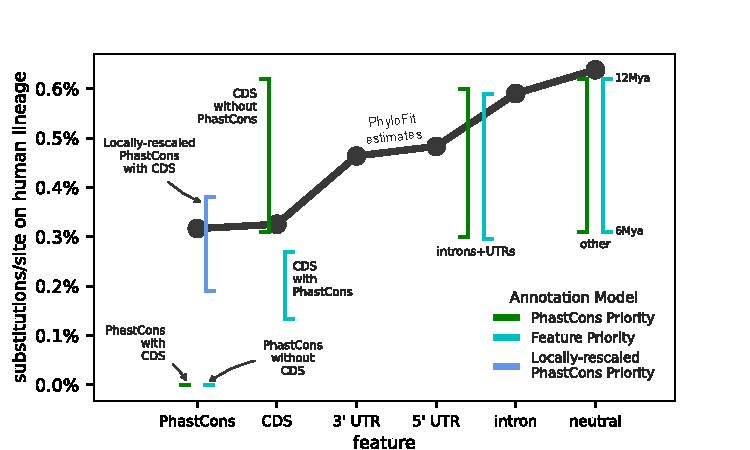
\includegraphics[width=\textwidth]{figures/figure_7_mod.pdf} 

    \caption{}

  \label{fig:figure-6}
\end{figure}

Since our B' method is based upon quantitative genetic models of linked
selection that explicitly incorporates the substitution process, fitting our
model to genomic diversity data leads to additional predictions. In particular,
our model predicts (1) the substitution rates per segment, (2) the fitness
variance per segment, and (3) the total number of strongly deleterious
mutations per diploid genome per generation. Given predicted substitution rates
for each feature can be compared to estimated sequence divergence between
species, this offers a qualitative check our model is producing sensible
results. 

To compare our models' predicted substitution rates against observed
divergence, we estimated sequence divergence on the human lineage using a
multiple alignment of five primates for each feature in our feature-based
models (Methods \ref{sec:methods-sub}). We compared these to the predicted
substitution rates per feature, averaging over all segments in the genome.
Since our simulations show that mutation rate estimates can be biased, we
predicted substitution rates under a fixed mutation rate of $\mu = 1.5 \times
10^{-8}$. Fixing the mutation rate also allows us to more easily compare the
predictions across our feature-based models. Unfortunately, a careful
comparison between our predictions and observed divergence rates is hindered by
considerable uncertainty in the rate of the molecular clock, generation times,
and the human-chimpanzee divergence time. We assume a generation time of 29
years, and calculate the sequence divergence implied by our predicted
substitution rates over a range of divergence times, from 6 Mya to 12 Mya
\parencite{Moorjani2016-tb,Nachman2000-te,Yi2002-pw,Steiper2006-xx}.

We find that our predicted substitution rates are qualitatively consistent with
the observed divergence along the human lineage for all features except
PhastCons (Figure \ref{fig:figure-7}). As expected, the predicted substitution
rates in features unlikely to be under selective constraint (introns and UTRs,
and the ``other" feature) are very close to the mutation rate. Throughout, we
report our substitution rates as a percent relative to the total mutation rate,
$\mu$ (here fixed to $1.5 \times 10^{-8}$). In our Feature Priority model,
coding sequences are predicted to have a substitution rate of 41.20\% of the
mutation rate, introns and UTRs 94.71\%, coding sequences 0\%, and the ``other"
feature 99.98\%. For comparison, the substitution rates along the human lineage
(as a proportion to the substitution rate in putatively neutral regions) are
74.15\% in UTRs, 92.44\% in introns, 50.96\% in coding sequences, and 49.56\%
in PhastCons regions. The large discrepancy between predicted and observed
PhastCons substitution rates is driven by our DFE estimates suggesting that the
bulk of mass is on selection coefficients greater than $10^{-3}$, which have no
chance of fixation in a population of $N_e \approx 10,000$. We note that our
DFE estimates are qualitatively similar to those inferred using the classic BGS
model; thus this DFE-substitution rate contradiction is not unique to our
estimates, and could indicate a potential model misspecfication problem.

\section*{Locally-rescaled Fits}

Given the observed DFE-substitution rate contradiction and that our simulations
indicated that $B(x)$ is more accurately predicted when we use local-rescaling,
we modified our composite-likelihood method to so that it can be run a second
time, on B' maps locally-rescaled by the predicted $\widehat{B}(x)$ from the
initial fit. Intuitively, this is based on the notion that if a neutral allele
experiences an effective population size of $B(x)N$, so too should a selected
allele, and this should be considered in how the SC16 equations are solved.
There is an important caveat about this analysis. Since local-rescaling is done
using the first round of maximum likelihood estimates, there is a possibility
of some circularity, since the $B(x)$ at this position includes the
contribution of the focal segment that is being rescaled. However, the results
do not change based on whether the $B(x)$ is at averaged at the 1 kbp level or
at the megabase scale; for the latter, a single segment makes little
contribution to the average. 

With this caveat noted, there are five important but tentative results to draw
from this analysis. First, the estimated mutation rate is implausibly higher,
reaching the upper limit of our optimization boundary of $\mu = 8 \times
10^{-8}$ across all populations in or PhastCons Priority model (Supplementary
Material XXX). When we re-ran optimization with an upper limit of $\mu = 1
\times 10^{-7}$, the mutation rate was again estimated to this (implausibly
large) upper limit, with no considerable changes to model fit or DFE estimates.
Second, all of our leave-one-chromosome-out $R_\text{LOCO}^2$ are about one
percentage point higher than the unrescaled model. This improved fit could be
an artifact of the circularity, so it is unimportant. Third, the DFE estimates
for PhastCons regions is now U-shaped (Supplementary Materials Figure
\ref{suppfig:rescale-dfe}), with $75-77\%$ of mass being placed on a weakly
deleterious class, $s=10{^-5}$. Interestingly, this is the first of all of our
models where such an appreciable mass has been placed on a midpoint in our
grid; in all other cases, non-strongly estimates were neutral ($s=10^{-8}$).
Fourth, predicted pairwise diversity is nearly identical to our original,
non-locally-rescaled fit (see Supplementary Materials Figure
\ref{suppfig:rescale}). Finally, since local-rescaling increases the DFE mass
over $s < 10^{-3}$, mutations in PhastCons regions now have the possibility of
fixation. We find that local-rescaling the PhastCons Priority, leads the
predicted substitution rates in PhastCons regions to be much closer to observed
levels (blue line, Figure \ref{fig:figure-6}).

Finally, as a robustness check, we investigated the extent to which
local-rescaling differed from the B' maps across selection parameters. We find
minor differences between the locally-rescaled and standard B' maps in the $0.2
\le 2N_e s \le 2$ range; the maps were identical under strong selection ($2N_e
s= 20$) as expected (Supplementary Materials Figure \ref{suppfig:rescale-b}).
Overall, this suggests that models that fit the linked selection are worryingly
sensitive the theoretic B' values in the $2Ns \le 1$ domain. Local-rescaling
turns out to only slightly alter the B' maps, yet significantly modifies the
DFE estimates. This brings the deleterious substitution rate in agreement with
observations (since this is predicted with a fixed $\mu = 1.5 \times 10^{-8}$;
however, the maximum likelihood estimate of mutation is implausibly high.

\section*{Discussion}

Linked selection processes alter genetic diversity on multiple scales, creating
patterns based on their strength relative to the stochasticity of coalescence
times and mutations. Sweeps typically leave signals on shorter genomic scales
(i.e. kilobases; \cite{Akey2004-zg}) which combined with the paucity of
adaptive substitutions in humans suggests positive selection is generating the
apparent large, megabase-scale linked selection signal
\parencite{Hernandez2011-gs,Murphy2022-sj}. By contrast, there is reasonable
evidence that negative selection against new mutations occurring in
highly-conserved sequences is generating large-scale chromosomal patterns of
diversity. 

Population genetic theory has been productively applied to fit this linked
selection signal, producing plausible estimates of the strength of selection at
these conserved regions and mutations rates consistent with more precise
pedigree-based estimates. However, these models rely on the canonical
background selection model, which due to its assumption that mutations are
sufficiently deleterious they cannot fix, has constrained statistical methods
to only fit background selection models in regions \emph{a priori} under
constraint. In reality, the relationship between diversity levels and the
strength of selection at deleterious mutations is U-shaped, which implies there
could be more uncertainty that previously appreciated in the distribution of
weak and strongly deleterious mutations.

We sought to address this uncertainty in this work, by leveraging a different
class of linked selection models based on modeling the equilibrium fitness
variance \parencite{Santiago2016-mu}. This model is more general than classic
background selection theory; the background selection model is analytically a
special case when the deleterious substitution rate is zero. Moreover, the SC16
model explains equilibrium fitness variance across all selection coefficients
by jointly predicting another central quantity in evolutionary genomics: the
deleterious substitution rate in conserved features. This offers a further way
to confirm or falsify that our understanding of the negative selection process
is accordance with other observed quantities.

However, while our improved negative selection model leads to nearly identical
parameter estimates as previous working employing classic BGS theory, we find a
fundamental contradiction in the implied rate of deleterious substitution and
observed divergence in conserved regions. Unfortunately, this suggests a
potentially serious model misspecfication or non-identifiability issue. Since
the rate of substitutions is determined by the fraction of DFE mass below $2N_e
s \le 1$, the consistency between our DFE estimates and those from
\textcite{Murphy2022-sj} suggests this discrepancy is shared across models of
negative selection.

One clue towards solving this contradiction is given by our simulation work.
While our linked selection model accurately predicts the substitution rates,
fitness variance, and diversity for $2N_e s > 1$ and $2N_e s \ll 1$, there's a
nominal error around the drift boundary of $2N_e s \approx 1$. This region of
parameter space is at a delicate balance between stochasticity dominating
allele frequency dynamics (for $2N_e s \ll 1$) and having little influence
($2N_e s > 1$). Our implementation of the SC16 model in essence only considers
the reduction due to selection \emph{within} the segment and not neighboring
regions. Thus, like classic BGS methods, our model does not consider selective
interference due to neighboring regions under selective constraint. Solving the
SC16 equations using a locally-rescaled population size of $B(x) N$ rather than
$N$ are in effect approximating the reduction in effective population due to
selective interference. Intuitively, this is based on the notion that if a
neutral allele experiences an effective population size of $B(x)N$, so too
should a selected allele. We find in simulations this reduces error around $2
N_e s \approx 1$. Unfortunately, employing this in our composite-likelihood
method would create some circularity, since the local $B(x)$ experienced at a
conserved segment includes the reduction due to the segment itself. There are
not computationally feasible ways to avoid this issue in the current
implementation.

Out of curiosity, we experimented with fitting human diversity data, using the
predicted $\widehat{B}(x)$ for local-rescaling, and rerunning our
composite-likelihood framework (see Supplementary Mathematical XXX). While the
circularity issue means these results should be interpreted with caution, we
generally find these models fit nearly as well 

it creates a bit of circularity. 



draft limits discussion - we were heavily constrained by simulations / regions
etc

the PhastCons Priority Model is very close to CADD 6\%, and interpretable,
similiar mutation rates. This 

weak selection remains elusive

UTR rates 

- parametric DFEs are trash

- the $pi_0$ problem

Ipsita Agarwal article 

what time scale is the average mutation being lost at?

Regularization / overfitting 

It is worth considering why this model performs well for models of negative
selection. The fitness variance equation, $V(x) = (U-2R)s$ tells us that under
models, the long-run variance is set by the balance of mutation and fixation.
Whether a particular basepair's behavior follows this equation depends upon
whether the long-run average is close to ``typical" for that basepair at a
given time. Good things fix so quickly, that we're left with a constant
churning of new variation

- need for coalescent simulations with reduced $N_e$ along the genome.

- we need to talk about Fisher's Fundamental Theorem and how this model
connects fitness variation to absolute changes in fitness.

Measuring selection in the Genome Versus Finding Selection in the Genome


\section*{Methods}
% (the method would support a new
% ``interaction" type, but this greatly increases the number of parameters).

\subsection*{Solving the B' Equations for each Segment}
\label{sec:methods-bprime-eqns}

Our software \texttt{bgspy} first calculates the equilibrium additive genic
fitness variation $\widetilde{V}_a$ and ratchet rate $\widetilde{R}$ for each
user-specified segments in the genome. These equilibria are calculated across
grids of mutation rate weighted by the DFE $m_i$ and selection coefficient
$s_j$, by numerically solving the following system of equations,

\begin{align}
  \label{eq:}
  {N}_{d} &= N \exp \left( -V_a \frac{Q^2(m_i, s_j)}{2} \right) & \text{\emph{effective population equation}} \\
  R &= \frac{4N_dU s_j}{\exp(4 N_d s_j)-1}  & \text{\emph{substitution equation}} 
\end{align}

where,

\begin{align}
  %V(x) &= U s - 2 {R}(x) s & \text{\emph{fitness variance equation}} \\
  V_a &= (U - 2 R) s_j & \text{\emph{fitness variance equation}} \\
  Q^2(m_i, s_j) &= \frac{2}{(1-Z)(2-(2-M)Z)} & \text{\emph{linkage inflation factor}} \\
  Z &= 1 - \frac{Us_j}{U-{M}} & \text{\emph{variance decay rate}}
\end{align}
%
and $U = m_i L$ and $M = r_\text{BP} L$ are the total mutation and
recombination rates in the segment. A detailed derivation of these equations
can be found in Supplementary Materials Section \ref{supp:theory}. The recombination
rate in a segment is determined by a user-supplied recombination map.

\subsection*{Calculating the Reduction Maps}
\label{sec:methods-maps}

Our method uses the pre-computed equilibria $\widetilde{V}_{a,g}$ for each
segment $g$ to calculate the reduction map $B(x; m_i, s_j)$ at positions $x$
across the parameter grids described above. Since we assume multiplicative
fitness, the reduction is the product of each segment's contribution accounting
for the recombination is,

\begin{align}
    B(x; m_i, s_j) = \exp\left(- \frac{1}{2}\sum_{g \in G} \sum_{i=1}^{n_s} \widetilde{V}_{a,g}(m_i, s_j) Q_g^2(m_i, s_j, r_{x, g})\right)
\end{align}
%
where $r_{x, g}$ is the recombination fraction between the focal site and
segment $g$. Here, $Q^2(m_i, s_j, r_{x,g})$ is given by Equation \eqref{eq:Q}
squared. A separate reduction map is calculated for all features $G$ within a
specific feature type. We calculate B' calculate for $\log_{10}$-spaced grids
over $10^{-1} \le s \le 10^{-8}$ and $10^{-11} \le m \le 10^{-7}$, in 10kb
increments across the genome.

\subsection*{Composite Likelihood and Optimization}
\label{sec:methods-likelihood}

Following previous approaches
\parencite{McVicker2009-ax,Elyashiv2016-vt,Murphy2022-sj}, we use a composite
likelihood approach to fit our negative selection model. Per-basepair allele
count data (described below) is summarized into the number of same and
different pairwise differences per window. All of our primary models were fit
with megabase windows, since previous work has found the strongest selection
signal at this scale (we confirm this with one XXX fit at the $10^5$bp scale).

Our binomial likelihood models the number of different pairwise comparisons
observed per window given the total number of pairwise comparisons. The
binomial probability for window $b$ is $\bar{\pi}(b; \Psi) = \pi_0 \bar{B}(b;
\mu, \mathbf{W})$, where bars indicate averages over some bin width. The free
parameters $\Psi = \{\pi_0, \mu, \mathbf{W}\}$ are the expected diversity in
the absence of selection ($\pi_0$), the mutation rate ($\mu$), and the
distribution of fitness effects for the discretized selection grid and $K$
features ($\mathbf{W}$). The reduction at position $x$ is then,

\begin{align}
    \log\left(B(x; \mu, \mathbf{W}) \right) = - \frac{1}{2} \sum_{g \in G} \sum_{j=1}^{n_s} V_g(\mu W_{j, k(g)}, s_j) Q_g^2(m_i, s_j, r_{x, g}).
\end{align}
%
See Supplementary Materials Sections \ref{supp:data-summary} and
\ref{supp:likelihood} for more details.

Our method uses two tricks to improve optimization over the mutation and DFE
parameters. First, we find $B(x; \mu, \mathbf{W})$ is exponential over columns
of $\mu \mathbf{W}$, which allows for optimization over this smooth function
rather than the grid. Second, we use softmax to convert constrained
optimization over the DFE columns (which must sum to one) to unconstrained. We
tested multiple different optimization routines, finding that BOBYQA
outperformed alternatives \parencite{Powell2009-jm,Johnson2007-tl}. We
inspected and confirmed convergence with diagnostic plots finding stable optima
across 10,000 random starts (see Supplementary Materials Section
\ref{supp:optima}). We assessed model fit using out-sample predictive error,
calculated by leaving out a whole chromosome during fitting and predicting its
diversity. To calculate uncertainty, we used a block jackknife approach in 10
Mbp windows (Supplementary Materials Section \ref{supp:jackknife}).

\subsection*{Human Population Genomic Data}
\label{sec:methods-data}

Our analyses was conducted on the Yoruba (YRI), European (CEU), and Han Chinese
(CHB) reference samples individuals from the high-coverage 1000 Human Genomes
data aligned to GRCh38/hg38 \parencite{Byrska-Bishop2022-tn}. Since nucleotide
diversity is a ratio estimator, it can be biased when subtly different
filtering criteria are applied to variant and invariant sites. To prevent this,
we conducted our analyses on Genomic VCF (gVCF) files that contain genotype
calls for both variant and invariant sites \parencite{Illumina_Inc2020-dk}.
Then, we apply the same genotype filtering criteria to all called sites
(Supplementary Materials Section \ref{supp:filter}). We also applied sequence
accessibility masks that containing only non-repeat, non-centromeric sequence
that passed the 1000 Genomes strict filter
(\cite{1000_Genomes_Project_Consortium2015-mi}; Supplementary Material Section
\ref{supp:accessible}). Since our theory only considers the indirect effects of
linked selection on a site, we additionally masked sites that are likely under
direct selective constraint (see Supplementary Materials Section
\ref{supp:neutral}). Finally, for every basepair passing these filtering and
masking criteria, we counted the number of reference and alternative allele
counts (excluding all multiallelic, indel, and CNV variants).

For all of our main analyses, we used the recombination map from
\textcite{Halldorsson2019-ey} estimated from a trio-based design to avoid
circularity that could occur by using LD-based maps. We use Ensembl gene
annotation \parencite{Cunningham2022-vk}, a special CADD Score dataset with
McVicker B scores removed (to avoid circularity;
\cite{Kircher2014-bv,Rentzsch2019-lr}), and PhastCons regions
\parencite{Siepel2005-wh}.

\subsection*{Forward Simulations}
\label{sec:methods-sim}

We conducted forward simulations of negative selection on whole human
chromosomes to validate our method at two stages. First, we simulated negative
selection on chromosome 10 using a realistic recombination map and putatively
conserved features to confirm that our classic B and new B' maps matched the
average simulation reduction map across mutation and selection parameters.
Second, we evaluated our composite likelihood method by simulating negative
selection on the first five human chromosomes, across grids of fixed mutation
and selection parameters. We then combined these into a synthetic genome, and
overlaid mutations on the ARG. Then, we ran our likelihood methods on the
resulting allele count data to assess model accuracy. We ran additional
synthetic genome simulations like these to evaluate the impact of two model
violations: recessivity of deleterious mutations and expanding populations. For
the latter, after $9.3$ generations, we grew the population by factor of 1.004
each generation to mimic the human expansion out-of-Africa
\parencite{Gutenkunst2009-pg}. We did not simulate population bottlenecks since
our analyses showed little difference between bottlenecked out-of-Africa
samples (CEU and CHB) and YRI samples. More details about these and the segment
simulations shown in Figure \ref{fig:figure-1}A-C can be found Supplementary
Section \ref{supp:simulation}.

\subsection*{Substitution Rate Estimation and Prediction}
\label{sec:methods-sub}

We estimated the divergence along the human branch using PhyloFit
\parencite{Siepel2004-ql} run on the Multiz alignments
\parencite{Blanchette2004-bb} of humans and four other primates (\emph{Pongo
abelii}, \emph{Pan troglodytes}, \emph{Pan paniscus}, \emph{Gorilla gorilla}).
PhyloFit was run using the HKY85 substitution model per-feature; estimates from
alternate substitution models yielded equivalent results. Further details about
this process can be be found in the GitHub repository
(\url{https://github.com/vsbuffalo/bprime}).

\printbibliography

\end{document}
